\documentclass[11pt]{beamer}
\usepackage[polish]{babel}
\pagestyle{empty}
\usepackage{minted}
\usepackage[T1]{fontenc}
\usepackage{amsmath}
\usepackage{amsfonts}
\usepackage{amssymb}
\usepackage{graphicx}
\title{Porównanie wydajności oraz ocena łatwości w użyciu wybranych narzędzi programowania równoległego.}
\author{Rafał Lenart}
\graphicspath{ {./images/} }

\begin{document}

\maketitle
\begin{frame}
	\tableofcontents
\end{frame}

\section{Wstęp}
\subsection{Cel projektu}
\begin{frame}{\subsecname}

	Celem przeprowadzanej oceny jest określenie przypadków użycia oraz ewaluacja 
	użyteczności  i wydajności wybranych narzędzi 
	służacych do programowania równoległego. Szczególnej uwadze zostanie poddana biblioteka distributed-ranges z pakietu oneAPI firmy Intel. 

	Opinia ta zostanie wydana na podstawie implementacji wybranych algorytmów i pomiarze 
	wydajności czasowej i pamięciowej programów. 
	Dodatkowo,	zważając na fakt, iż jedną z głównych intencji twórców biblioteki distributed-ranges, która będzie głównym kandydatem do porównania, jest 
	usprawnienie procesu pisania kodu dla programistów, krytyce zostanie poddana łatwość 
	pracy z danym narzędziem oraz ilość napisanego kodu.
	
\end{frame}

\subsection{Plan działania}
\begin{frame}{\subsecname}
	\begin{enumerate}
		\item Wybór podobnych do siebie technologii/narzędzi użytych do porównania.
		\item Dobór algorytmów do implementacji.
		\item Implementacja, pisanie kodu.
		\item Pomiar prędkości oraz zużycia pamięci. Wyznaczenie innych kryteriów oceny takich jak ilość linijek kod lub porównanie czasu jaki zajęło pisanie i zrozumienie danego narzędzia.
		\item Dokonanie porównania technologii z wzięciem pod uwagę wszystkich kryteriów. 
	\end{enumerate}	
\end{frame}

\section{Użyte technologie}
\begin{frame}
	\begin{center}
	\usebeamerfont{title}\insertsectionhead\par%
	\end{center}
\end{frame}

\begin{frame}{\secname}
Wyborem technologii do porównania kierowało podobieństwo przypadków użycia. Jako, że biblioteka distributed-ranges służy do programowania systemów z pamięcią rozproszoną, pozostałe narzędzia również będą pracować na pamięci rozproszonej. Narzędziem które jest używane wewnątrz biblioteki jest model SYCL który również będzie brany pod uwagę. 
\end{frame}

\subsection{SYCL}
\begin{frame}{\subsecname}
SYCL jest modelem programowania pozwalającym aplikacji na przełączanie i współpracę pomiędzy różnymi akceleratorami sprzętowymi takimi jak CPU, GPU i FPGA (bezpośrednio programowalne macierze bramek).

Model ten dostarcza warstwę abstrakcji ułatwiającą używanie ujednoliconej pamięci współdzielone (Unified Shared Memory).

\end{frame}

\subsection{distributed-ranges}
\begin{frame}{\subsecname}
Biblioteka distributed-ranges to twór bazujący na SYCL  oraz wprowadzonej w standardzie C++ bibliotece ranges.

Celem twórców narzędzia jest usprawnienie pracy z pamięcią rozproszoną podczas programowania systemów z wieloma GPU/CPU z równoczesnym utrzymaniem wydajności podobnej do modelu SYCL.
\end{frame}

\subsubsection{ranges}
\begin{frame}{\subsubsecname}
Range (z ang., zakres) - to struktura posiadająca początek i koniec (begin() i end()) udostępniająca ustandaryzowany sposób iterowania po jej wartościach.
Standard C++20 udostępnia kilka konceptów posiadających rózne cechy. na przykład random\_access\_range lub contiguous\_range.
\begin{figure}[h]
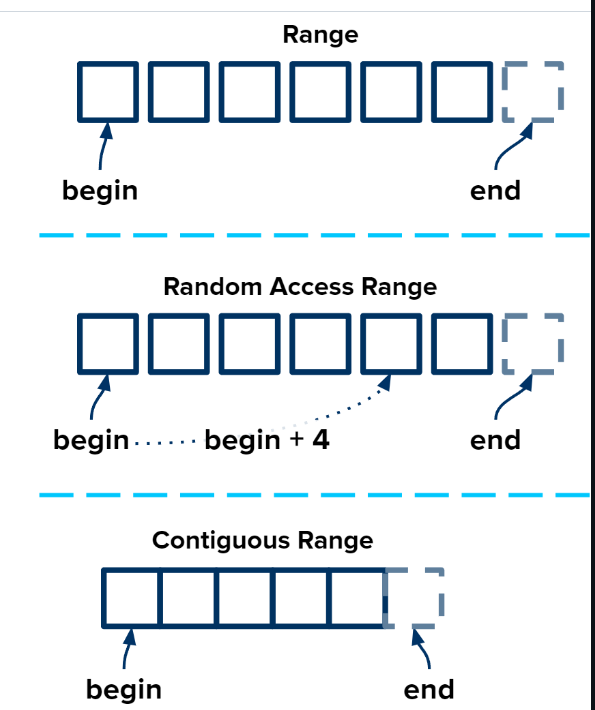
\includegraphics[scale=0.25]{ranges}
\end{figure}
\end{frame}

\subsection{MPI}
\begin{frame}{\subsecname}
Message Passing Interface (MPI, z ang., interfejs transmisji wiadomości) to standard przesyłania komunikatów między procesami programów równoległych. Jest on obecnie dominującym modelem wykorzystywanym w superkomputerach. MPI umożliwia pracę na rozproszonych systemach pamięci.
\end{frame}

\section{Wybrane algorytmy}
\begin{frame}
	\begin{center}
	\usebeamerfont{title}\insertsectionhead\par%
	\end{center}
\end{frame}

\subsection{Radix-2 FFT}
\begin{frame}{\subsecname}
	Szybka transformata Fouriera Radix-2 to algorytm który dzieli wektor wejściowy na dane indeksowane parzyście i te indeksowane nieparzyście. Po podziale dla obu wektorów obliczana jest wartość dyskretnej transformaty Fouriera po czym wyniki są łączone w całość. Ważnym ograniczeniem algorytmu jest to, że dla $n$ będącego wielkością wektora wejsciowego prawdziwe jest $$x \in \mathbb{N}$$ $$n = 2^x$$ \\
	Zastosowana metoda "dziel i zwyciężaj" sprawia, że algorytm jest dobrym kandydatem do zrównoleglania.
\end{frame}

\begin{frame}{\subsecname}
Wzór dyskretnej transformaty Fouriera
$$\sum_{n=0}^{N-1}{x(n)e^{-j2\pi kn/N}}$$
\end{frame}

\begin{frame}[containsverbatim]{\subsecname}
	\begin{exampleblock}{Przykład pseudokodu wykonania algorytmu:}
	\end{exampleblock}
\begin{minted}[fontsize=\scriptsize]{python}
import cmath
def radix2(vec):
  n = length(vec)
  if n <= 1:
	return x
  # Podział na dwie równe części	
  even = radix2(vec[0::2])
  odd = radix2(vec[1::2])
  # Łączenie rezultatów
  for k in range(n // 2):
	t = cmath.exp(-2j * cmath.pi * k / n) * odd[k]
	vec[k] = even[k] + t
	vec[k+n // 2] = even[k] - t
  return vec
		
	
	
\end{minted}
\end{frame}

\subsection{Algorytm QR Obliczania wartości własnych}
\begin{frame}{\subsecname}
	Dla $A \in \mathbb{C}^{n\times n}$ liczba $\lambda \in \mathbb{C}$ to wartość własna macierzy a niezerowy wektor $x \in \mathbb{C}^n$ jest wektorem własnym, jeśli $$Ax = \lambda x$$
liczby $\lambda$ to pierwiastki wielomianu charakterystycznego macierzy A.	Widmem macierzy nazywamy zbiór jej wartości własnych

\end{frame}

\begin{frame}{\subsecname}
	Macierze $Q, R \in \mathbb{R}^{n\times n}$ tworzą rozkład QR macierzy $ A \in \mathbb{R}^{n\times n}$ kiedy $$A = QR$$
R jest macierzą trójkątną górną natomiast Q jest macierzą ortogonalną.
\begin{figure}[h]
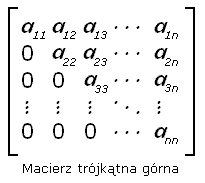
\includegraphics[scale=0.5]{macierz-trojkatna-gorna}
\end{figure}
\end{frame}

\begin{frame}{\subsecname}
Macierz ortogonalna to taka macierz kwadratowa $A \in M_n(\mathbb{R})$ która spełnia równość $$A^{-1} = A^T$$ 
\begin{figure}[h]
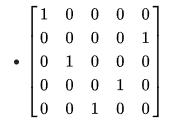
\includegraphics[scale=1]{macierz-ortogonalna}
\end{figure}
\end{frame}

\begin{frame}{\subsecname}
Macierz Hessenberga - to taka macierz trójkątna górna która bezpośrednio pod diagonalą posiada dodatkową przekątną.
\begin{figure}[h]
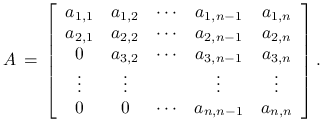
\includegraphics[scale=0.5]{macierz-hessenberga}
\end{figure}
Dowolną macierz można przekształcić do tej postaci metodą Householdera
\end{frame}

\subsubsection{metoda Householdera}
\begin{frame}[containsverbatim]{\subsubsecname}

\begin{minted}[fontsize=\scriptsize]{python}
import numpy as np

def householder(A):
    m, n = A.shape
    Q = np.eye(m)

    for k in range(min(m-1, n)):
        x = A[k:, k]
        # Wektor Householdera
        v = x - np.linalg.norm(x) * np.eye(len(x), 1, 0)
        H = np.eye(m)
        H[k:, k:] -= 2 * np.outer(v, v) / np.linalg.norm(v)**2
        A = H @ A
        Q = Q @ H

    return Q, A
\end{minted}

\end{frame}

\begin{frame}[containsverbatim]{\subsecname}

\begin{minted}[fontsize=\scriptsize]{python}
def qr_iteration(A, max_iter=1000, tol=1e-6):
    Q, R = np.linalg.qr(A)

    for i in range(max_iter):
        A = np.dot(R, Q)
        Q, R = np.linalg.qr(A)

        # Sprawdzamy warunek stopu
        if np.abs(np.diag(A) - np.diag(R * Q)).max() < tol:
            break

    eigenvalues = np.diag(A)
    return eigenvalues
\end{minted}
\end{frame}

\subsection{Conjugate Gradient}
\begin{frame}{\subsecname}
	Metoda gradientu sprzężonego (ang. conjugate gradient method) jest algorytmem służącym do rozwiązywania niektórych układów równań liniowych. można nią rozwiązywać układy których macierz jest symetryczna i dodatnio określona. Jest metodą iteracyjną.
\end{frame}


\end{document}